\documentclass[a4paper]{ctexart}
\usepackage[margin=2cm]{geometry}
\usepackage{amsmath}
\usepackage{tkz-euclide}
\usepackage{paralist}
\usepackage{fancyhdr}\pagestyle{fancy}
\fancyhead[]{}
\fancyhead[C]{启航培优}
\fancyfoot[C]{第\thepage 页}
\ctexset{
    section/format = \youyuan \huge \centering \vspace{1em},
    subsection/name = {,、\hspace{-1em}},
    subsection/format = \heiti \zihao{4} \raggedright ,
    subsection/number = \chinese{subsection},
    subsection/indent = 1.67\ccwd
}
\newcounter{liti}
    \newenvironment{xt}{\begin{list}{\arabic{liti}.}{\usecounter{liti}%
        \labelsep=2ex
        \itemindent = 4\ccwd
        \listparindent = \parindent
        \leftmargin = 0cm
        \rightmargin = 0cm
        \itemsep=2cm
    }}{\end{list}}
\newcommand{\tk}{\underline{\hspace{6\ccwd}}}
\begin{document}
    \section*{冬令营刷题4}
    \subsection{填空题}
    \begin{xt}
        \item 计算:$\dfrac{2\dfrac{1}{4}+0.25}{2\dfrac{3}{4}-\dfrac{1}{2}}+\dfrac{2\times 0.5}{2\dfrac{1}{5}-\dfrac{2}{5}}=$ \tk.
        \item 某月里,星期五、星期六和星期日各有5天,那么该月的第1日是星期\tk.
        \item 大于$\dfrac{1}{2016}$ 且小于$\dfrac{1}{2015}$ 的真分数有\tk 个.
        \item 哥哥和弟弟各买了若干个苹果,哥哥对弟弟说:“若我给你一个苹果,咱俩的苹果个数一样多”,弟弟想了想,对哥哥说:“若我给你一个苹果,
        你的苹果数将是我的2倍”,则哥哥与弟弟共买到了\tk 个苹果.
        \item 如图,$AB=AD$,$\angle DBC=21^\circ $,$\angle ACB=39^\circ$,则$\angle ABC=\tk $度.
        \begin{flushright}
            \begin{tikzpicture}
                \tkzDefPoints{0/0/A,3/0/B}
                \tkzDefPointBy[rotation = center A angle 60](B) \tkzGetPoint{D}
                \tkzDefPointBy[rotation = center B angle -21](D) \tkzGetPoint{c}
                \tkzInterLL(A,D)(B,c) \tkzGetPoint{C}
                \tkzDrawPolygon(A,B,C)
                \tkzDrawSegments(B,D)
                \tkzLabelPoints[right](B,C)
                \tkzLabelPoints[left](A,D)
            \end{tikzpicture}
        \end{flushright}
        \vspace{-2cm}
        \item 己知抽水机甲和抽水机乙的工作效率比是3:4,如两台抽水机同时抽取某水池,15小时抽干水池.现在,乙抽水机抽水9小时后关闭,
        再将甲抽水机打开,要抽干水池还需要\tk 小时.
        \vspace{1cm}
        \item $n$为正整数,形式为$2^n-1$的质数称为梅森数,例如:$2^2-1=3$,$2^3-1=7$是梅森数.最近,美国学者刷新了最大梅森数,$n=74207281$,
        这个梅森数也是目前己知的最大的质数,它的个位数字是\tk .
        \item 图中,$ABCD$是直角梯形,上底$AD=2$,下底$BC=6$,$E$是$DC$上一点,三角形$ABE$的面积是15.6,三角形$AED$的面积是4.8,
        则梯形$ABCD$的而积是\tk .
        \begin{flushright}
            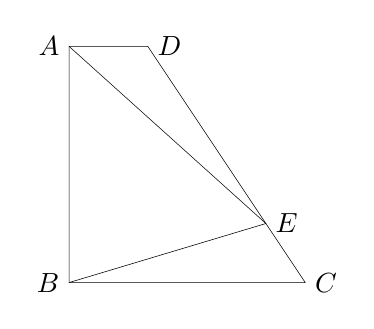
\begin{tikzpicture}
                \tkzDefPoints{0/0/B,3/0/C,0/3/A,1/3/D}
                \tkzDefPointBy[homothety = center C ratio .25](D) \tkzGetPoint{E}
                \tkzDrawPolygon(A,B,C,D)
                \tkzDrawSegments(B,E A,E)
                \tkzLabelPoints[right](C,D,E)
                \tkzLabelPoints[left](A,B)
            \end{tikzpicture}
        \end{flushright}
    \subsection{解答下列各题(要求写出简要过程)}
        \vspace{-2cm}
        \item 甲、乙两人,在一圆形跑道草上同时同地出发,反向跑步.己知甲的速度是每分钟180m,乙的速度是每分钟240m,在30分钟内,它们相遇了24次,
        问跑道的长度最多是多少米?\vspace{5cm}
        \item 一筐苹果分成甲乙两份,甲的个数和乙的苹果个数比是27:25,甲多乙少,若从甲中至少取出4个,加入乙中,则乙多甲少,问这筐苹果有多少个?
        \vspace{5cm}
        \item 右图是一个等边三角形,等分为4个小的等边三角形,用红和黄两种颜色涂染它们的顶点,要求每个顶点必须涂色,且只能图一种颜色.涂完后,
        如果经过旋转,等边三角形的涂色相同,则认为是相同的涂色,则共有多少种不同的涂法?
        \begin{flushright}
            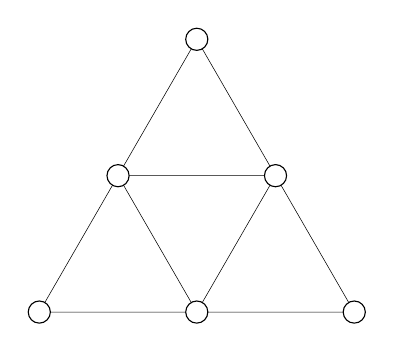
\begin{tikzpicture}
                \tkzDefPoints{0/0/A,2/0/B,4/0/C}
                \tkzDefPointBy[rotation = center A angle 60](B) \tkzGetPoint{D}
                \tkzDefPointBy[rotation = center B angle 60](C) \tkzGetPoint{E}
                \tkzDefPointBy[rotation = center D angle 60](E) \tkzGetPoint{F}
                \tkzDrawPolygon(A,B,D)
                \tkzDrawPolygon(B,C,E)
                \tkzDrawPolygon(D,E,F)
                \tkzDrawPoints[size=8,fill=white](A,...,F)
            \end{tikzpicture}
        \end{flushright}
        \item 三台车床$A$,$B$,$C$各以一定的工作效率加工同一种标准件,$A$车床比$C$车床早开机10分钟,$C$车床比$B$车床早开机5分钟,$B$车床
        开机10分钟后,$B$,$C$车床加工的标准件的数最相同.$C$车床开机30分钟后,$A$,$C$两车床加工的标准件个数相同.$B$车床开机多少分钟后就
        能与$A$车床加工的标准件的个数相同?\vspace{3cm}
    \subsection{解答下列各题(要求写出详细过程)}
    \vspace{-2cm}
        \item 黑板上先写下一串数:1,2,3,…,100,如果每次都擦去最前面的6个,并在这串数的最后再写上擦去的6个数的和,得到新的一串数,再做同
        样的操作,直到黑板上剩下的数小足6个.问:
        \begin{asparaenum}[(1)]
            \item 最后黑版上剩下的这些数的和是多少?
            \item 最后所写的那个数是多少?
        \end{asparaenum}
        %(1)(2)
        \vspace{10cm}
        \item 数学竞赛,填空题8道,答对1题,得4分,未答对,得0分;问答题6道,答对1题,得7分,未答对,得0分.参赛人数400人,
        至少有多少人的总分相同?
    \end{xt}

\end{document}